\section{OpenETCS Tool Chain Characteristics}
\label{sec:toolchain-analysis}

All the methods mentioned above start with a complete definition of the toolchain. In OpenETCS, the development of the toolchain follows an \emph{agile} approach.
Hence, for each (major) release we have to deal with an incomplete tool
chain. In addition to the methods of the previous section,  we need a qualification
process that can adapt to the development speed, deal with an incomplete toolchain
and can re-use qualification information.


Moreover, as stated by Asplund et al., the toolchain itself may
provide some mechanisms that may reduce the tool qualification effort
\cite{asplund_towards_2012,asplund_qualifying_2012}. They are
described as a set of safety goals that the tool chain should ensure.
 In our context, most of the
tool integration effort is made by integrating tools into a tool
platform.  According to Asplund et al., the tool platform should
ensure the following safety-goals that will avoid some extra tool qualification:
\begin{itemize}
\item Coherent time stamp information: common time stamps on development artifacts.
\item Notification: the user should be notified when artifacts changed.
\item Data integrity:  avoid use of obsolete artifacts, the data used reflects the
  current state.
\item Data mining: all data used by safety analysis should be available and be
  verifiable.
\end{itemize}

These goals will be included in our tool integration
qualification, they will be extra requirements for each tool qualification.
Moreover, a set of specific requirements has been described in the
deliverable D2.6 \cite{baro_d2.6_2013}. These should also been
included in the tool's requirements.

In the following sections we define the tool chain qualification
process by first giving an overview of the process (section
\ref{sec:process_overview}), then getting into details for individual
tool qualification (section \ref{sec:individual-tool-qualif}), we then
focus on the incremental development of the tool chain (section
\ref{sec:incremental}) and finally provide some example on how this process can be applied to our tool
chain implementation (section \ref{sec:toolchain-qualification-process} ).

\section{Qualification Process Overview}
\label{sec:process_overview}
Figure \ref{fig:qualification_process} defines the qualification
process.

\begin{figure}[htbp]
\begin{center}
\scalebox{0.9}{
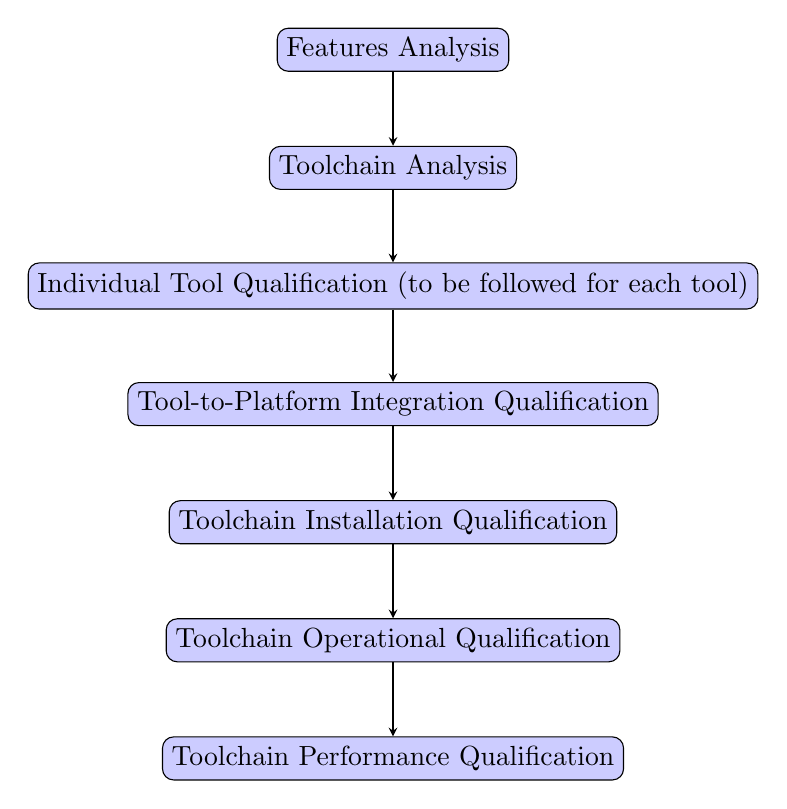
\begin{tikzpicture}[->, >=stealth,node distance=1.5cm, auto]
\tikzstyle{decision} = [diamond, draw, fill=blue!20, align=center, font=\footnotesize]
\tikzstyle{block} = [rectangle, draw, fill=blue!20, align=center, rounded corners]
	\node [block] (n1) {Features Analysis};
	\node [block, below of=n1] (n2) {Toolchain Analysis};
	\node [block, below of=n2,align=center] (l1) {Individual Tool
          Qualification (to be followed for each tool)};
        \node [block,below of=l1] (n9) {Tool-to-Platform Integration Qualification};
	\node [block, below of=n9] (n10) {Toolchain Installation Qualification};
	\node [block, below of=n10] (n11) {Toolchain Operational Qualification};
	\node [block, below of=n11] (n12) {Toolchain Performance Qualification};

	\draw[->] (n1) -- (n2);
	\draw[->] (n2) -- (l1);
	\draw[->] (l1) -- (n9);
        \draw[->] (n9) -- (n10);
	\draw[->] (n10) -- (n11);
	\draw[->] (n11) -- (n12);
\end{tikzpicture}}
\end{center}
\caption{Proposal for the openETCS qualification process}
\label{fig:qualification_process}
\end{figure}



The steps of the process are defined as follows:

\paragraph{Feature Analysis}
The tool chain is defined as feature or activity (e.g. ``Requirements
Engineering'', ``Documentation'', ``Modelling'') . Each tool of the
tool chain  is then categorised according to its activities. Inside
a feature  a work-flow is defined.

This phase  also defines  the interfaces of each tool within a feature
and the artifacts manipulated. An artifact is defined by a name and a
format.


\paragraph{Tool chain Analysis}
The work-flow between the tool chain features is defined.
The interfaces between the features are defined at this phase as well as
the artifacts exchange between the different features.

\paragraph{Individual Tool Qualification (to be followed for each tool)}
See section \ref{sec:individual-tool-qualif}

\paragraph{Tool-to-Platform Integration Qualification}
This step ensures that the tool is correctly integrated within the tool chain.
After all individual tools are qualified, their integration into the
tool chain is planned. As part of the integration planning, the team
will analyse the dependencies of the different tools to minimise the
effects of unavoidable dependencies.

Moreover, for each artifact used or produced by the tool, evidence
should be provided that the safety-goals of section
\ref{sec:toolchain-analysis} are satisfied. 
Whenever an artifact is modified, a new time stamp has to be added and
notification should be triggered. Whenever an artifact is used a check
of its obsolescence should be performed.

\paragraph{Tool Chain Installation Qualification}
Installation should verify that the toolchain is properly
installed. It does not verify that the tool chain conforms to the functional and performance specification. This is done later in the operational qualification phase. The goal of this step is to verify correct software installation and to document all computer hardware, software and configuration settings as the initial baseline configuration.

\paragraph{Operational qualification}
Operation qualification should demonstrate that the tool chain will function according to its operational specification in the selected environment. The tests should be performed to verify that the toolchain meets the specifications, requirements in the specific environment.

\paragraph{Performance qualification}
Performance qualification should demonstrate that the toolchain consistently performs according to the specifications defined by the openETCS project, and is appropriate for the intended use. Important for consistent openETCS toolchain performance is regular preventive maintenance, making changes to the toolchain in a controlled manner and regular testing.

The toolchain should be well maintained to ensure proper ongoing performance. Procedures should be in place for regular preventive maintenance of it to detect and fix problems before they can have a negative impact.

\section{Individual Tool Qualification}
\label{sec:individual-tool-qualif}
The qualification of a tool chain implies that each tool should be
qualified. Figure \ref{fig:tool_qualification_process} proposes a tool
qualification process that should be performed for each tool.
This section explains the steps for the tool qualification whenever a
new tool is added. Next section will deal with the special cases where tools are
updated and when a first qualification has already been performed.

\begin{figure}[htbp]
\begin{center}
\scalebox{0.9}{
\begin{tikzpicture}[->, >=stealth,node distance=1.5cm, auto]
\tikzstyle{decision} = [diamond, draw, fill=blue!20, align=center, font=\footnotesize]
\tikzstyle{block} = [rectangle, draw, fill=blue!20, align=center,
  rounded corners]
	\node [align=center] (l1) {Individual Tool Qualification (to be followed for each tool)};
        \node [block, below of =l1] (n3) {Define Process \& Usage Context};
	\node [block, below of=n3] (n4) {Tool Classification};
	\node [decision, below of=n4, anchor=north] (d1) {Tool is\\prequalified};
	\node [below of=d1, node distance = 3cm] (subd1) {};
	\node [block, left of=subd1, node distance=4.5cm] (n5) {Check conformance\\with defined process\\and usage context};
	\node [decision, right of=subd1, node distance=4.5cm] (d2) {Qualification\\by third party\\possible};
	\node [block, below of=d2, node distance=3cm] (n6) {Provide process and usage context\\for third party qualification};
	\node [decision, below of=d1, node distance= 3cm] (d4) {Conformance?};
	\node [decision, below of=d4, node distance=3cm] (d3) {Tool is\\open source\\or T1 or T2?};
	\node [below of=d3, node distance = 2.53cm] (subd3) {};
	\node [block, fill=red!20, right of=subd3, node distance=2.5cm] (n7) {Qualification difficult\\(possibility: e.g., ``proven in use'')};
	\node [block, left of=subd3, node distance=2.5cm] (n8) {Operational Qualification\\by Tool Chain Integrator};
	\node [block, below of=d4, node distance=8cm] (n9) {Tool-to-Platform Integration Qualification};
	\begin{scope}[on background layer]
		\node [block, fill=black!10, fit=(l1) (n3) (n4) (d1) (n5) (d2) (n6) (n9)] (individual_quali) {};
	\end{scope}
	\draw[->] (n3) -- (n4);
	\draw[->] (n4) -- (d1);
	\draw[->] (d1) -- node [near start] {yes} (n5);
	\draw[->] (d1) -- node [near start] {no} (d2);
	\draw[->] (d2) -- node [near start] {yes} (n6);
	\draw[->] (d2) -- node [near start] {no} (d3);
	\draw[->] (d3) -- node [right] {no} (n7);
	\draw[->] (d3) -- node [left] {yes} (n8);
	\draw[->] (n5) -- (d4);
	\draw[->] (d4) -- node [near start] {no} (d2);
	\draw[->,dashed] (n7) -- (n9);
	\draw[->] (n8) -- (n9);
	\draw[->, out=190, in=180] (d4) to node [near start] {yes} (n9);
	\draw[->, out=-50, in=0] (n6) to (n9);


\end{tikzpicture}}
\end{center}
\caption{Proposal for the openETCS Tools qualification process}
\label{fig:tool_qualification_process}
\end{figure}

\subsection{Define Process \& Usage Context}
The process starts by defining the tool purposes and the usage context
of tool. More precisely, the formats restrictions of the input and
output artifacts  of the tool should be identified, the dependency with
our tools should be explicitly defined and the feature analysis should
be consolidate. This can be best achieved in a model-based manner.
For details on that topic please refer to
Section~\ref{sec:model-based-tool-quali}.

\subsection{Tool Classification}
The class of the tool should be set according to the EN50128
definition (see section \ref{sec:sota-tool-qualification} ). An evidence can be expressed using the feature and
the tool chain analysis.


These two first steps may be seen as pre-qualification steps that
guides the qualification process.

\subsection{Scenario-based Qualification of Individual Tools}
\label{sec:scenario-based-tool-quali}


Qualifying a toolchain always requires the qualification of the individual tools it is comprised of. The effort required depends on the type and license of the tool to be qualified. To this end in the following we have identified a number of different scenarios that are of relevance in the context of the openETCS project as depicted in Figure~\ref{fig:tool-qualification-scenarios}.

\begin{figure}[htbp]
\begin{center}
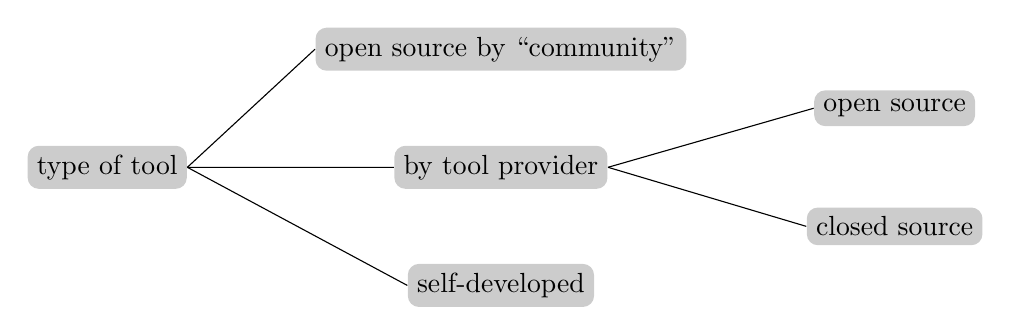
\begin{tikzpicture}[parent anchor=east,child anchor=west,grow=east, edge from parent, level distance=5cm]
	\tikzstyle{every node}=[fill=black!20,rounded corners]
	\node {type of tool}
		child { node {self-developed} }		
		child { node {by tool provider}
			child { node {closed source} }
			child { node {open source} }
		}
		child { node {open source by ``community''} };
\end{tikzpicture}
\end{center}
\caption{Scenarios to consider when qualifying individual tools}
\label{fig:tool-qualification-scenarios}
\end{figure}

In the following considerations for the individual scenarios are described.

\subsubsection{Self-developed Tool}

For a self-developed tool the project needs to provide the means for qualification and quality assurance. As the tool has not been employed in productive use by others the ``proven in use'' argument (CENELEC EN50128 §6.7.4.4 a)) does not apply.

\subsubsection{Tool Provided by a Tool Provider}

For tools provided by a third party we must distinguish again two cases:

\paragraph{The tool is provided as closed source tool}

If the tool is not pre-qualified by the tool provider the options are limited for T3 tools. If the tool provider is not willing or unable to provide the means for qualification, the qualification of a T3 tool will be difficult. One possibility is the ``proven in use'' argument: if the tool is already in use on a broad scale in industry and is generally regarded as reliable for the intended purpose this can be sufficient. This situation is represented as the red node in the process graph in Figure~\ref{fig:tool_qualification_process}.

\paragraph{The tool is provided as open source}

In this case it would be possible to adapt the tool and analyse it to enable qualification. However, this involves a huge amount of effort which is best done by the tool provider who as a better insight into the tool's internal workings. Also a third party who has already experience with the tool or is a specialist with regards to qualifying safety-critical tools could be entrusted with the qualification task.

\subsubsection{Open Source Tool Provided by the ``Community''}

If no tool provider can be identified but the tool is developed by the community and distributed under an open source license, the tool qualification has to be conducted by the project. However, many open source tools have a large development and expert community which can certainly be of help. In addition, the ``proven in use'' argument could possibly be applied (e.g., for tools like GCC).

\subsection{Model-based Tool Qualification}
\label{sec:model-based-tool-quali}

This section describes a proposal on how to setup the operational qualification of individual tools. This step of the qualification process (cf. Figure~\ref{fig:tool_qualification_process}) is required for any tool that is not pre-qualified. With respect to the scenarios described in Section~\ref{sec:scenario-based-tool-quali} it applies to self-developed and third party tools classified T1 and T2 and open source T3 tools. In the case of closed source T3 tools it is not possible to follow this process as the internal workings of the tools are hidden.

We propose setting up the operational tool qualification based on the approach by Slotosch et al. which has been briefly sketched in Section~\ref{sec:slotosh-approach}. It has been simplified and adapted to our purposes. In particular, we will focus on the artifacts and documentation necessary to conduct the qualification steps. Figure~\ref{fig:qualification-models-linkage} shows the different parts of the qualification model according to \cite{slotosch_model-based_2012}. We propose to tailor this approach as follows:
\begin{itemize}
    \item The different levels of requirements have been simplified: We propose to keep a single level of requirements. In addition we distinguish two special types of requirements: the \emph{use cases} and \emph{safety requirements} which are derived from a safety standard such as CENELEC EN~50128. Safety requirements often enforce constraints to the development process and the employed methods and do not necessarily specify desirable properties of the end result.
    \item In the context of openETCS the tool design model is built using SysML with the Papyrus tool. 
	\item The ``Quality Assurance'' part, containing existing problem reports, their severity and relations to tests and potential errors, can be covered by using the GitHub issue tracker and is therefore not depicted in Figure~\ref{fig:qualification-models-linkage}.
\end{itemize}

\begin{figure}[htbp]
\begin{center}
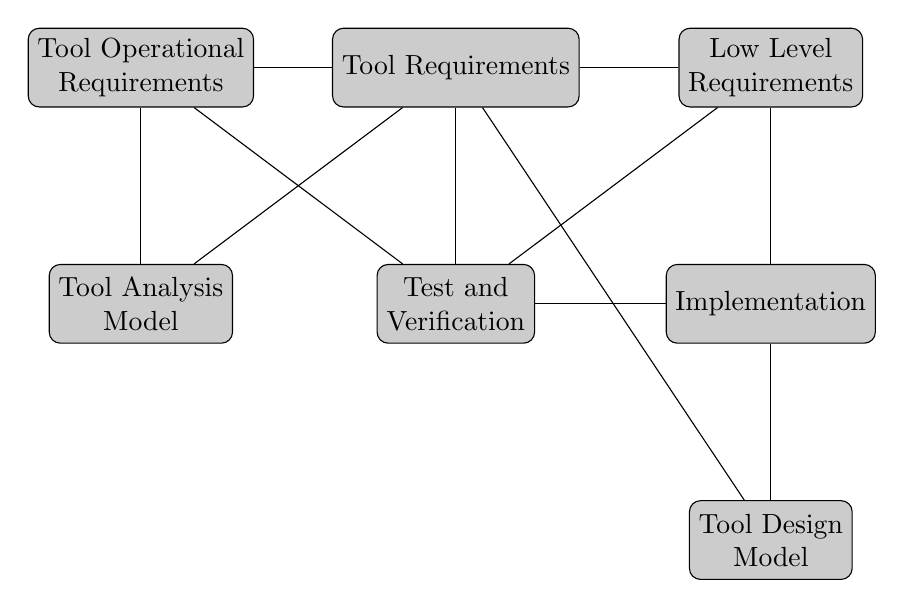
\begin{tikzpicture}
	\tikzstyle{block} = [rectangle, draw, align=center, minimum width=2cm, minimum height=1cm]
	\node[block] (n1) at (0,0) {Tool Operational\\ Requirements};
	\node[block] (n2) at (4,0) {Tool Requirements};
	\node[block] (n3) at (8,0) {Low Level\\Requirements};
	\node[block] (n4) at (0,-3) {Tool Analysis\\Model};
	\node[block] (n5) at (8,-6) {Tool Design\\Model};
	\node[block] (n6) at (8,-3) {Implementation};
	\node[block] (n8) at (4,-3) {Test and\\Verification};
	\draw (n4) -- (n1);
	\draw (n4) -- (n2);
	\draw (n1) -- (n2);
	\draw (n2) -- (n3);
	\draw (n3) -- (n6);
	\draw (n2) -- (n5);
	\draw (n5) -- (n6);
	\draw (n8) -- (n1);
	\draw (n8) -- (n2);
	\draw (n8) -- (n3);
	\draw (n8) -- (n6);
\end{tikzpicture}
\end{center}
\caption{Parts of the qualification model and their linkage according to \cite{slotosch_model-based_2012}}
\label{fig:qualification-models-linkage}
\end{figure}

The SysML block diagrams depicted in Figure~\ref{fig:tool_analysis_model} depicts the proposed qualification meta-model for openETCS. It needs to be instantiated for each individual tool. The tool analysis model is used to analyse the functions of the tool and potential errors and mitigations. Ideally, it shall establish the traceability between requirements, use cases, implementations and test cases.


\begin{figure}
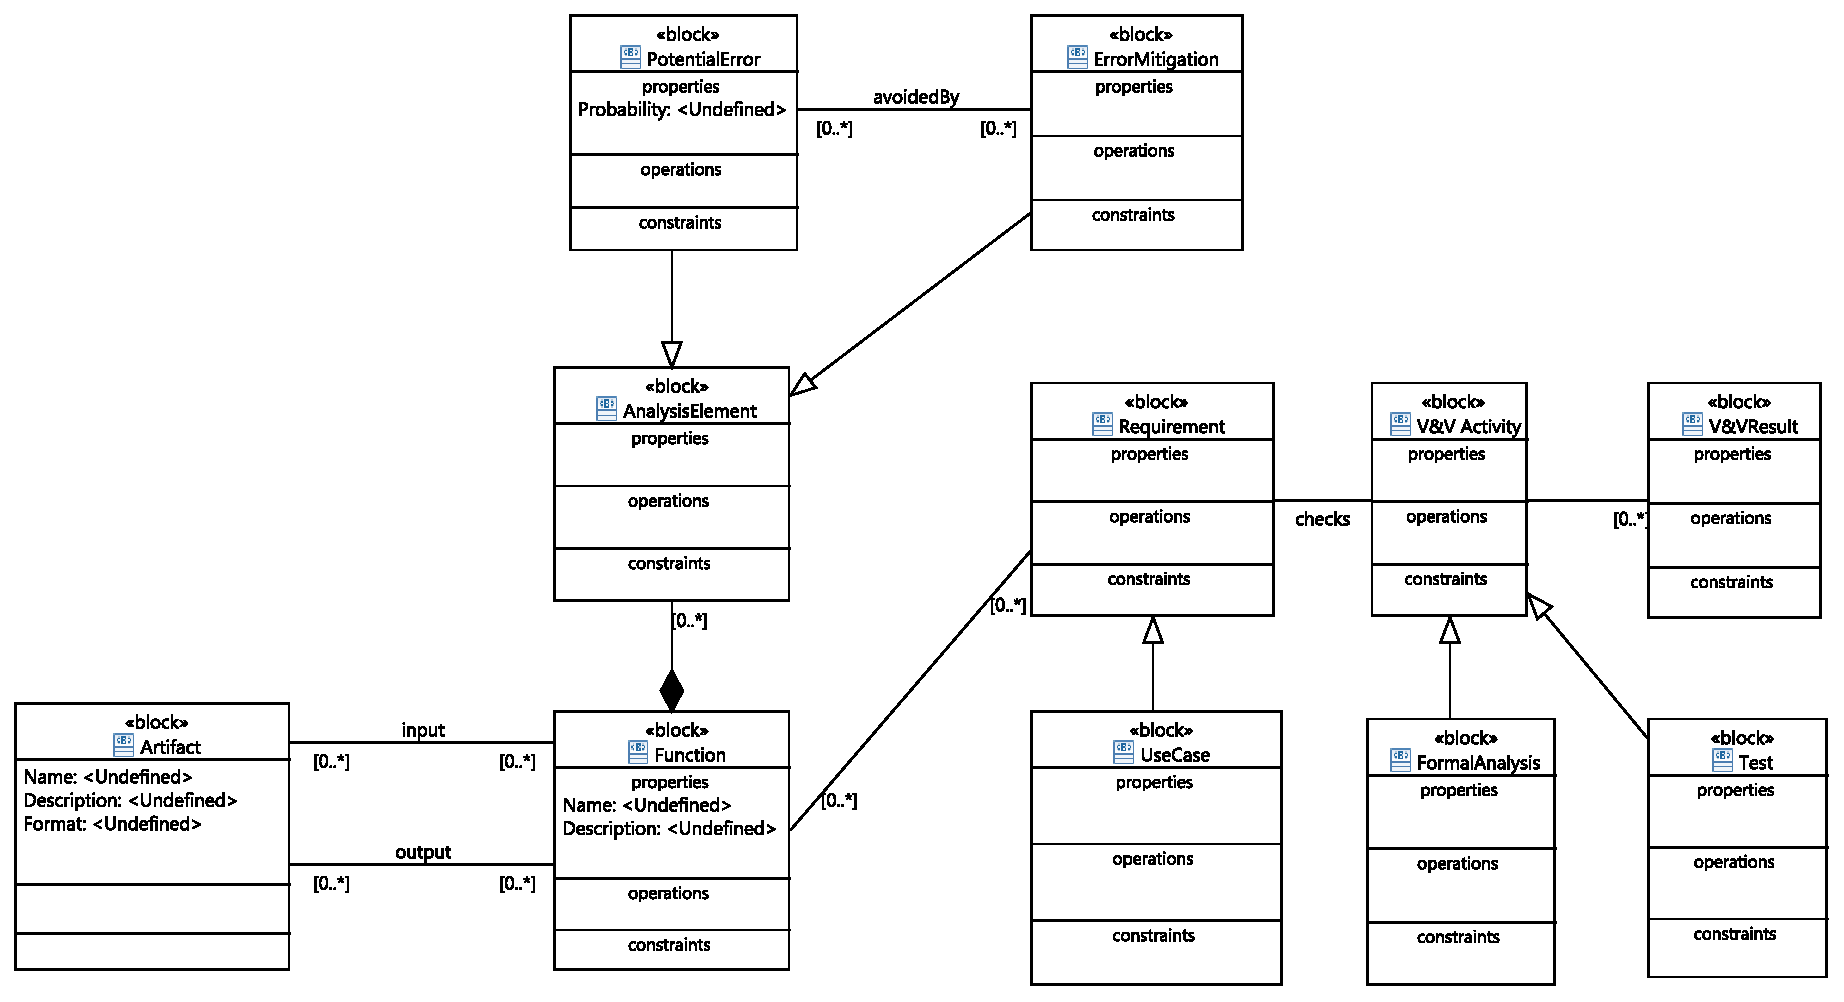
\includegraphics[width=\textwidth]{ToolAnalysisModel.pdf}
\caption{Tool analysis meta model for qualification}
\label{fig:tool_analysis_model}
\end{figure}


Each tool will then be defined by all information represented in our
meta-model. This can be seen as our template for collecting all
information needed for tool qualification.



\section{Incremental Tasks for toolchain qualification}
\label{sec:incremental}

The qualification of the toolchain shall follow an incremental process
adding the next tool to the previously qualified tool chain. The
process will continue until the last qualified tool is integrated and
the complete toolchain is qualified. A bottom-up approach will be
applied. As a result, the errors related to tool interface should be
easier to pinpoint.

A new  OpenETCS tool chain release deal with different type of changes:
\begin{enumerate} 
\item Add a new tool: the tool chain is extended
\item Replace a tool: a tool function is replaced by another one
\item Update a tool: a tool is update (bug fixes, performance
  improvements ...)
\end{enumerate}

In the first case, the complete qualification process should be
performed and the qualification of the new tool should be added.

In the two other cases, the feature model should also be updated, as
well as the manual, the use cases and the potential  errors.
Moreover, evidence that all tools that depend on this tool are still
compatible with the new one.  

In all cases of a new qualification  the three last phases should also be
performed again.

During the toolchain qualification there will be iterative tasks where
users repeat a set of actions over and over again. Thus, it would be
necessary to evaluate these type of tasks and try to automate a subset
of them to minimise the execution time.


\section{OpenETCS Toolchain Qualification Process}
\label{sec:toolchain-qualification-process}

This section will apply the set of concepts described in the previous
section to the openETCS tool chain.
Figure \ref{fig:openetcs-process} implements the qualification process
described in the previous section.

\begin{figure}[htbp]
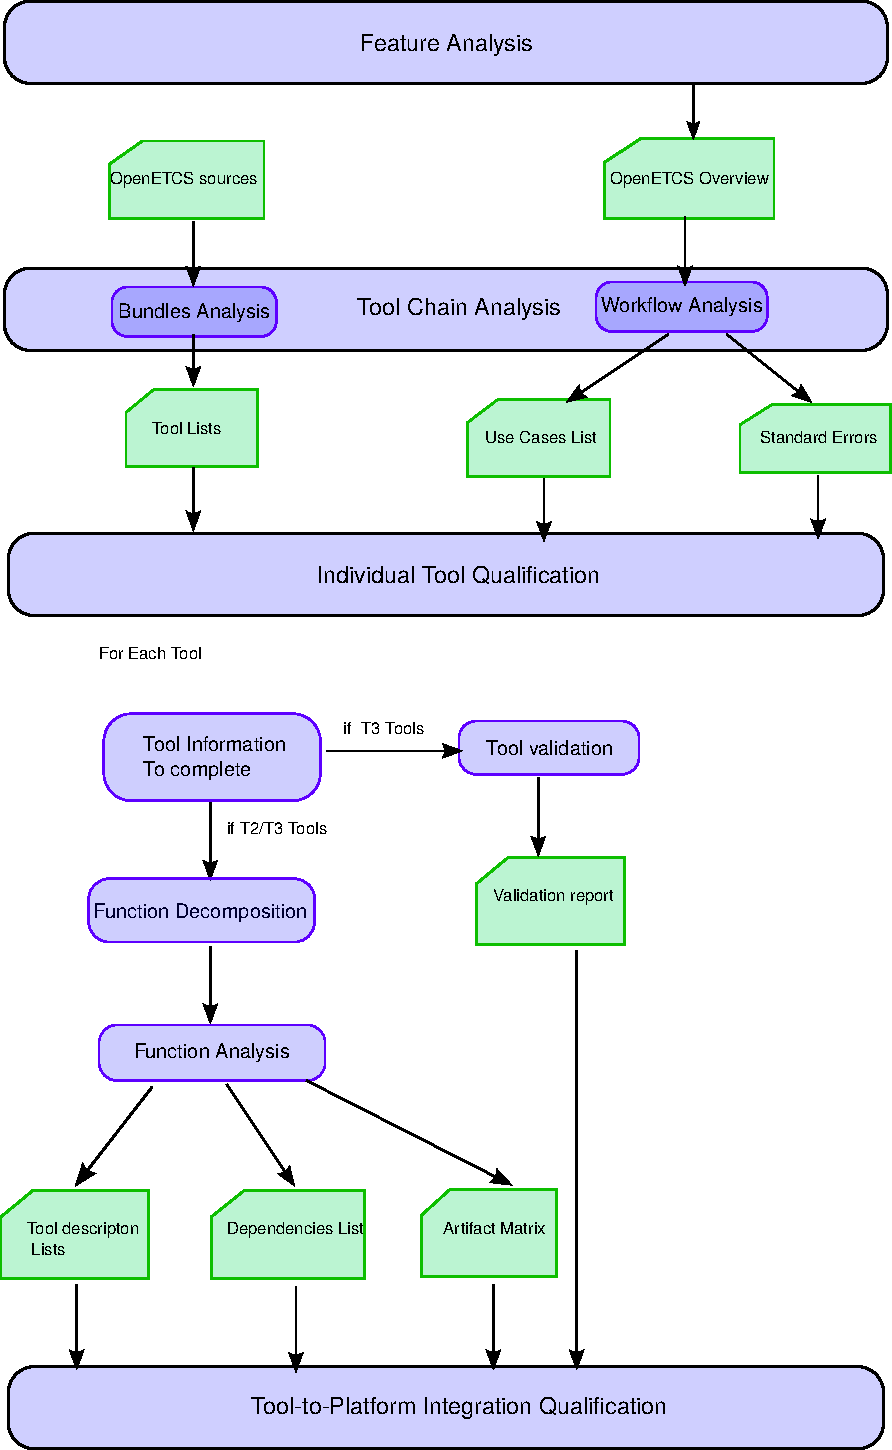
\includegraphics[width=\textwidth]{openETCS_process.pdf}
\caption{\label{fig:openetcs-process} The OpenETCS Qualification process}
\end{figure}

The first step is the {\bf feature Analysis}.
The OpenETCS tool chain  will be defined by the set of its features and
a guideline describing how to correctly use it.
A SysML block diagram describes the tool chain architecture at a certain point in time as shown in
Figure \ref{fig:overview}. 
\begin{figure}[htbp]
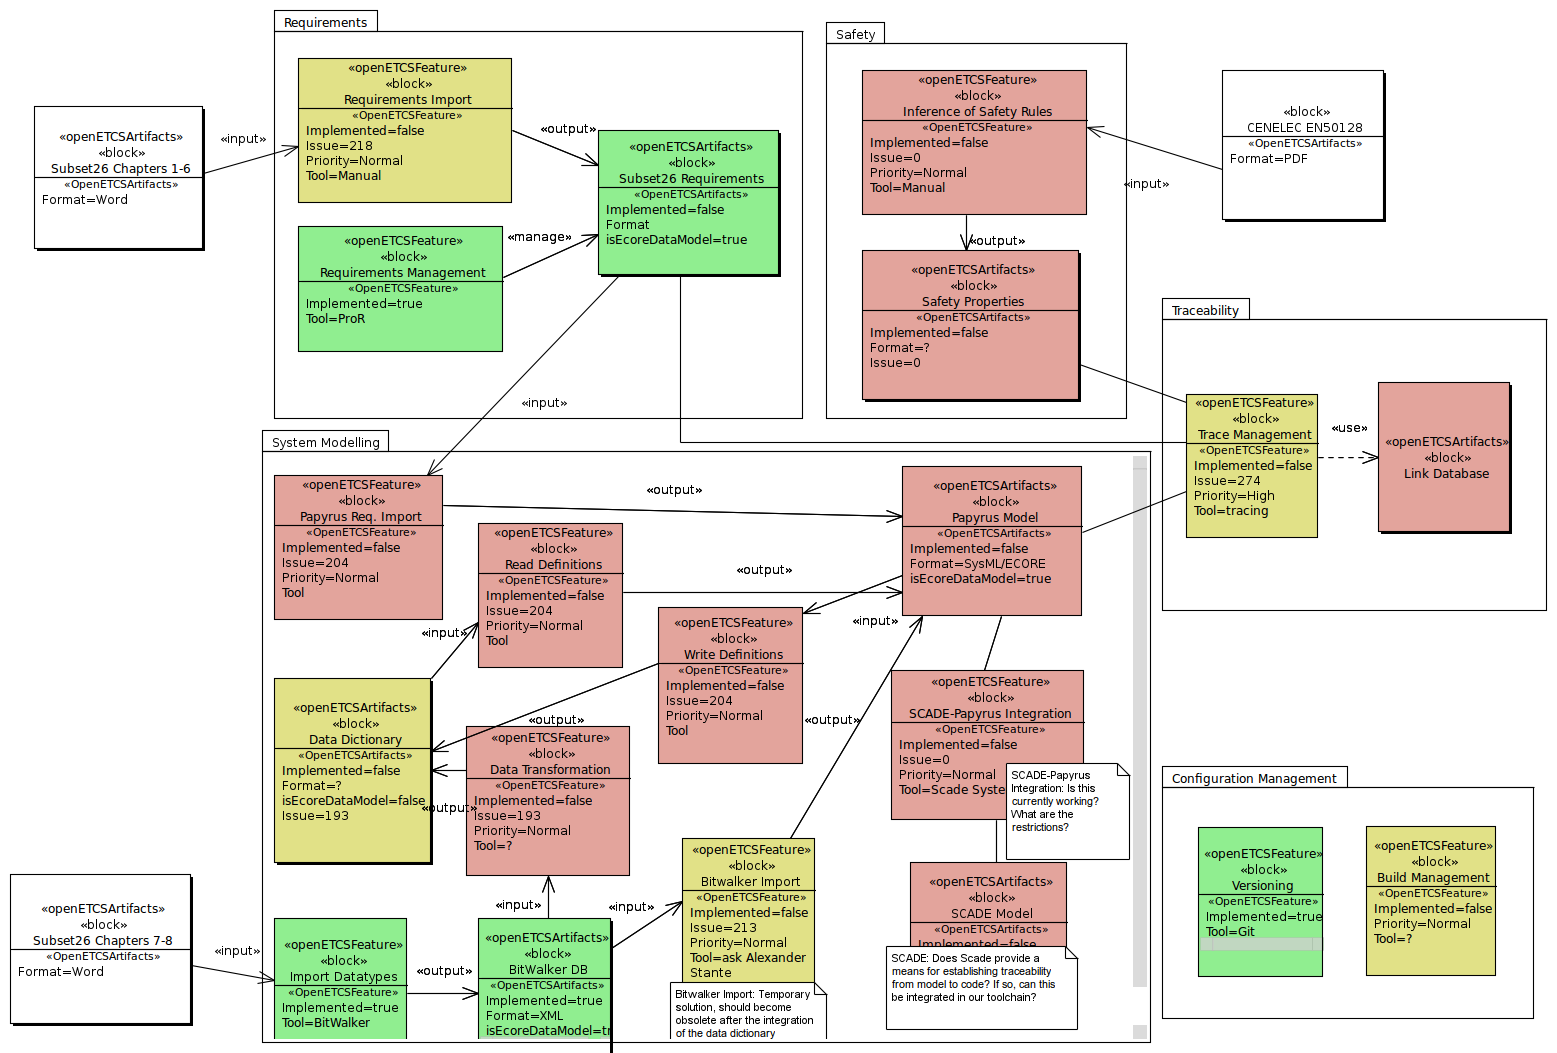
\includegraphics[width=\textwidth]{ToolChainmodel}
\caption{\label{fig:overview} Tool Chain overview (20.02.14) -- \\
  Green Block: Implemented \\
  Yellow Block: Work in Progress \\
  Red Block: Not started \\
  White Block: External Artifacts} 
\end{figure}
This block diagram is intended to grow according to new feature requests and the
needs of openETCS participants.  This diagram will be kept updated
as a reference of our tool chain. In any case, the complete information
regarding the feature availabilities  may be found in the Eclipse product
definition.

Each feature of the toolchain is a block with the profile ``openETCSFeature''
and  each artifact is block with the profile ``openETCSArtifact''.  Each
feature realises at least one use case and may be implemented by one or more tools.
Note that in the tool platform features  may also be
implemented as plug-ins. The diagram also imposes a (partial) order
on the tasks. While some may be done in parallel, many tasks are dependent on others.
Currently, the diagram neither highlights the use of the tools, nor the order of actions
to be performed. This diagram should be completed by guidelines on
how to use the tool chain and/or an activity diagram.

%To mitigate the qualification process, we will first consider more
%than one feature at a time considering that errors from a tool A may
%be detected by a Tool B in the next step of the tool chain process.
%Furthermore, the toolchain is a collection
%of features and not only tools. This differs from Asplund and al. in the sense that
%some of the tool integration mechanisms that automate transformation of data, represent features
% and are thus not out of the scope of the qualification.

%Due to our development process, a ``pre-qualification'' of tools should be made
%when integrating a tool.


The second step, the {\bf tool chain analysis} consists of Bundle Analysis
and the work-flow Analysis.
The openETCS tool chain is integrated into the Eclipse platform. One
can analyses the sources of the tool chain and automatically derived
the list of tools present in the tool chain as well as some
information about them such as :  the name,  the version,
a description and a list of dependency.
These information should be included in the release documentation of
the opentECTS tool chain.

The list of tool should be refined by the development team.
The missing information should be added directly in the
sources to make them available for the next tool releases.


From the work-flow of the tool chain it is possible to automatically
derived some basic use cases such as parsing or producing
artifacts. These basic use cases may be coupled with basic potential
errors such as ``no file found'', ``too many file produced''...

After the tool chain analysis phase, the {\bf individual tool qualification}
starts. With the help of the tool list, the previous information given
(from former releases) and the basic use cases, the tool information
should be completed. Table \ref{tbl:tool-info} \ref{tbl:artifacts} and
\ref{tbl:functions} summarise the set of information needed for the
qualification of a tool.



\begin{table}[htbp]
\centering
\caption{\label{tbl:tool-info}Tool Information to be completed}

\begin{tabular}{|l|p{5cm}|}\hline
Tool Name: & \\\hline
Version: & \\\hline
Tool License: & \\\hline
Tool Origin: &\\\hline
Tool Dependencies & \\
(with version) & -\\
 & -\\ \hline
Description: & \\
 & \\ \hline
Tool Class: & \\\hline
\multicolumn{2}{|c|}{If T2/T3 Tools}\\\hline
Tool Justification & \\
 & \\ \hline
Manual or Specification & \\
Link and version & \\\hline
Artifact List link & \\\hline
Function List link& \\\hline
\multicolumn{2}{|c|}{If T3 Tools}\\\hline
Evidence of correctness or  & \\
failure detection \footnotemark& \\\hline
VnV activities report link&\\\hline
\end{tabular}

\vspace{1em}
$^1$\footnotesize{See EN50128 6.7.4.4 for the list of alternatives}
\end{table}


\begin{table}[htbp]
\caption{\label{tbl:artifacts} List of  Artifacts Description}
{\small
\begin{tabular}{|p{4em}|l|p{1.5cm}|l|p{5em}|p{1.8cm}|l|p{5em}|}\hline
Name & Format & Is read ? By who ?& Restrictions & Time stamp check? &Is
written ? By Who ?& Restrictions & Time Stamp produced ?\\\hline
\multirow{2}{*}{Artifact1} & \multirow{2}{*}{tex} & Tool1 & none & yes &no & &\\\cline{3-8}
                           & & Tool2 & none& no & no & &\\\hline
\end{tabular}
}
\end{table}


\begin{table}[htbp]
\centering
\caption{\label{tbl:functions} Function Definition}
\begin{tabular}{|p{5cm}|p{5cm}|}\hline
Name&\\\hline
Description& \\\hline
Inputs & \\\hline
Outputs & \\\hline
Use Case & \\\hline\hline
Potential Errors & Error Mitigation \\\hline
&  \\\hline
&  \\\hline
\end{tabular}
\end{table}




When all tool are completely defined the {\bf tool-to-platform
  integration} starts. From the previous phases, we should be able to generate
the dependency list of the tools and the artifact matrix. The
dependency list is obtained by following the work-flow  and the
eclipse dependency list definition that includes the version of the tools.
The dependency list is used to check if
all tool can be correctly integrated into the tool platform by the
qualification team and report to the development team. Part of this
task may be automatically done by the Eclipse tool platform. 

The artifacts matrix is the list of all artifacts produce within the
tool chain with the link of each tool that uses, writes or reads it. 
As required by \tt{R-WP2/D2.6-02-076} the input/output formats has to
be documented.
The artifacts matrix  allows the qualification team to check if all artifacts are correctly
read and write and/or all possible errors are mitigated.  In case of
re-qualification of the tool chain, impact analysis of the change
shall be perform form the artifacts matrix. Hence,  the work may be
alleviate by focusing on the tools that are impacted by
the changes. 


%% \paragraph{Tool Integration Process for Qualification}

%% \begin{itemize}
%% \item Define name and version
%% \item Describe use cases
%% \item Provide justification of the tool within the tool chain
%% \item Provide input/output artifacts format (associated with the
%%   version)
%% \item Integrate the tool in the SysML model
%% \item Provide tool manual and other available documentation (associated with the version)
%% \item Link with an issue tracker
%% \end{itemize}

%% One possible implementation is to represent all these in formations
%% directly in the SysML model.

%% \todo[inline]{This high-level list should be detailed.  What I would expect: Which artefacts exist; How they are connected; When artefacts have to be re-validated (e.g. due to changes); What roles exist; who is responsible for what; etc.}
%% \paragraph{The Qualification Process}

%% \begin{enumerate}
%% \item Feature Analysis
%%   \begin{itemize}
%%   \item This step should assign a class to each feature based on the use cases.
%%   \item Define the potential errors
%%   \item Identify counter measure and/or error detection
%%   \item For T3 tools 2 alternatives:  certified compiler/generator or
%%     object code checker and/or exhaustive tester
%%   \end{itemize}
%% \item Tool platform  analysis 
%%   \begin{itemize}
%%   \item Provide evidence that the safety-goals mentioned in the
%%     previous sub-section are fulfilled\textcolor{red}{[The identification of safety goals is missing in step 1]}
%%   \end{itemize}
%% \item Toolchain Analysis
%%   \begin{itemize}
%%   \item Defines the work-flow
%%   \item Identify the ``hot spots'' of the toolchain
%%   \item Rearrange the toolchain if possible
%%   \item Find new measures when needed with combining tools (redundancy with orthogonal
%%     codes \ldots{})
%%   \end{itemize}
%% \item Toolchain qualification verification 
%%   \begin{itemize}
%%   \item Check consistency of tool version with  manuals and other
%%     provided feature information
%%   \item Generate table to  check if all possible errors has a
%%     detection or a correction mechanism
%% \item Generate the qualification report
%%   \end{itemize}

%% \end{enumerate}





%%  LocalWords:  openETCS opentECTS
